\chapter{Mathematical background}
The flow of CSF around the spinal cord requires equations for fluid flow to be coupled with equations for elasticity or in the optimal case, poroelasticity. The underlying concepts of these kinds of problems were originally developed somewhat independently within petroleum engineering, geomechanics and hydrogeology. The equations will first be presented separately. Later in the chapter, coupling conditions will be discussed. Several quantities will be discussed and as far as possible, we try to use a consistent notation for each quantity throughout the study. 
\\
\\
This chapter intends to give a short description of the mathematical theory behind modeling CSF. The equations are first introduced by assuming a fixed set of coordinates. Later, the two fundamental descriptions of motion are discussed. \\
\\
In providing the neccessary mathematical background it is convenient to give a overview of the notation used. If not specifically specified otherwise we use: \\ \\
$\mathbf{v}$ - Velocity of the material. In the fluid, $\mathbf{v}$ represents fluid velocity, and in the solid $\mathbf{v}$ denotes the velocity of the solid.
\\ \\
$ \mathbf{U}$ - Total displacement of the solid. In the fluid, this quantity represents the total mesh displacement. 
\\
\\
$p$ - Pressure in the fluid. In the case of elasticity, the same pressure does not exist in the solid, and in the case of poroelasticity $p$ represent the pore pressure inside the fluid/solid mixture. 
\\
\\
$\mathbf{w}$ - Domain velocity, (i.e, all material points within the domain moves with velocity $\mathbf{w}$). In the case of a pure elastic medium, the solid domain changes with the velocity of the solid, $\mathbf{v}$, so in the solid we have $\mathbf{v} = \mathbf{w}$ which will not neccessary hold in the fluid.
\\
\\
Unit vectors in the cartesian coordinate system are denoted $\mathbf{i} = (1,0,0), \mathbf{j} = (0,1,0)$ and $\mathbf{k} = (0,0,1)$. For summation convenction the common choice $\mathbf{i}_i, \mathbf{i}_j, \mathbf{i}_k$ are used respectively. 
\\
\\
The index notation to denote components of vectors and tensors are used together with Einstein summation convention $\mathbf{v}_i\mathbf{i}_i = v_1\mathbf{i}_i + v_2 \mathbf{i}_j + v_3 \mathbf{i}_k$ for a vector $\mathbf{v} = (v_1,v_2,v_3)$ are used ocasionally. A sum is taken over a repeated index. 
\\
\\
It should be noted that the definition of $\nabla$ differs in the literature. We define $\nabla$ as a tensor, $\nabla = \mathbf{i}_i\pdi{}{x_i}$, and thus $\nabla \mathbf{v} = \pdi{v_i}{x_j}\mathbf{i}_j\mathbf{i}_i$
\\
\\
Subscripts \textit{f} and \textit{s} are used to denote fluid and solid quantities, respectively
\section{Fluid flow}
The most fundamental equations in fluid flow are conservation laws. These equations are based on classical mechanics and states conservation of mass, momentum and energy. In the literature, these are often reffered to as balance equations.
\subsection{The Divergence Theorem}
The divergence theorem is result that relates the flow of a \textit{vector field} through a closed surface to the divergence of the vector field inside the surface. The theorem is usually credited to Green or Gauss, but other mathematicians also contributed (see e.g. \cite{Katz79} for a brief history) . The divergence theorem states that for a vector field $\mathbf{F}$ in a region $V_0$ bounded by a closed surface $S_0$
\begin{align}
\int_{V_0} \nabla \cdot \mathbf{F} \mathrm{d}V = \int_{S_0} \mathbf{F} \cdot \mathbf{n} \mathrm{d}S \label{DivVector}
\end{align}
where $\mathbf{n}$ is the outward unit normal on $S_0$. For a second rank \textit{tensor}, $\mathbf{T} = T_{ij}\mathbf{i}_i\mathbf{i}_j$ for $i,j = 1,2,3$, the divergence theorem becomes a vector equation, and will differ slightly with the tensor notation used in this thesis. We have 
\begin{align} 
\nabla \cdot \mathbf{T} = \mathbf{i}_i\pdi{}{x_i} \cdot T_{kj}\mathbf{i}_k\mathbf{i}_j = \pdi{T_{ij}}{x_i} \mathbf{i}_j
\end{align}
To ensure the divergence theorem to hold for each direction $\mathbf{i}_j$, the volume integral over this expression must equal the surface integral of 
\begin{align}
T_{ij} n_i \mathbf{i}_j = n_i \mathbf{i}_i \cdot T_{jk}\mathbf{i}_j \mathbf{i}_k = \mathbf{n} \cdot \mathbf{T}
\end{align}
And therefore, the divergence theorem for a second-rank tensor becomes
\begin{align}
\int_{V_0} \nabla \cdot \mathbf{T} \mathrm{d}V = \int_{S_0} \mathbf{n} \cdot \mathbf{T} \mathrm{d}S \label{DivTensor}
\end{align}
For a symmetric tensor, $\mathbf{n} \cdot \mathbf{T} = \mathbf{T} \cdot \mathbf{n}$ and we can use the form \eqref{DivVector}. However, when dealing with non-symmetric tensors the form \eqref{DivTensor} must be used. 

\subsection{Reynolds Transport Theorem}
The famous engineer and scientist Osbourne Reynold stated the general conservation law the following way \cite{Reyn1903}:
\\
\\
Any change whatsoever in the quantity of any entity within a closed surface can only be effected in one or other of two distinct ways:
\begin{enumerate}
\item it may be effected by the production or destruction of the entity within the surface, or
\item by the passage of the entity across the surface.
\end{enumerate}
\begin{center}
\begin{figure}[!ht]
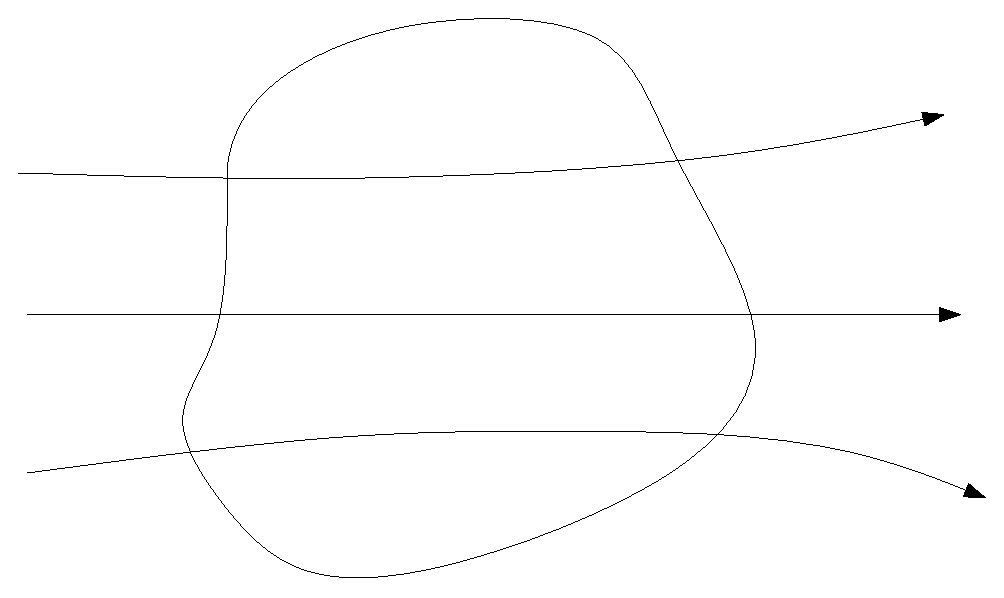
\includegraphics[scale=0.5]{figures/Fixed_control_volume} \\
\caption{Fixed control volume with flow as indicated by streamlines} 
\end{figure}
\end{center}
It should be noted that the transport theorem can be approached in two different ways. One for a fixed set of spatial coordinates, a fixed control volume, where fluid can enter and exit the boundaries of the defined body. The other approach has a control volume consisting of the same material particles at all times. Therefore the body has to follow the flow, and no fluid will cross the boundary. In this approach, one has to take into account the movement of the boundary of the body and the fact that the body can change it's volume. More on descriptions of motion is described in section \ref{sec:DoM}
\begin{center}
\begin{figure}[!ht]
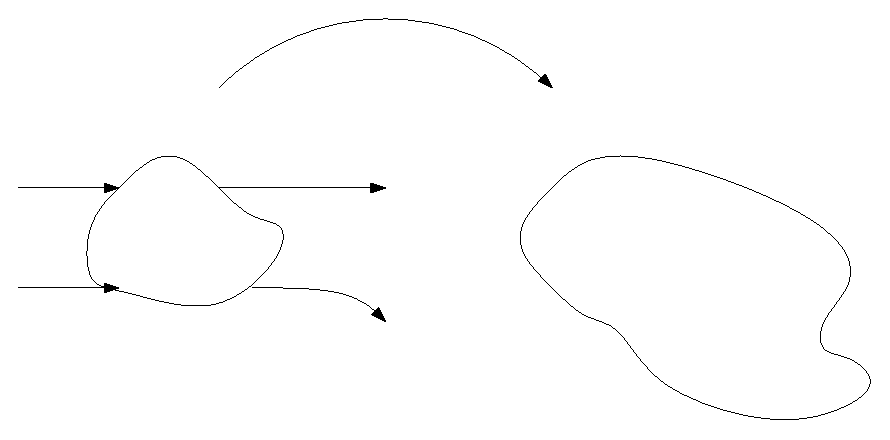
\includegraphics[scale=0.8]{figures/Moving_control_volume}\\
\caption{A moving control volume, consisting of the same fluid particles at time $t$ (left) and time $t+\Delta t$ (right) }
\end{figure}
\end{center}
Now, consider a fixed control volume, $V_0$ and some fluid property $Q(\mathbf{x},t)$. The rate of change of $Q$ within the control volume can be written
\begin{align}
\frac{\mathrm{d}}{\mathrm{d}t} \int_{V_0} Q(\mathbf{x},t) \, \mathrm{d}V \label{Rate_of_change}
\end{align}
The net change of $Q$ must be equal the rate of change in $Q$ within the control volume plus the net rate of mass flow out of the volume. In other words:
\begin{align}
\frac{\mathrm{d}}{\mathrm{d}t} \int_{V_0} Q(\mathbf{x},t) \, \mathrm{d}V = \int_{V_0} \pdi{Q(\mathbf{x},t)}{t} \mathrm{d}V + \int_{S_0} Q(\mathbf{x},t) \mathbf{v} \cdot \mathbf{n} \mathrm{d}S \label{Reynolds}
\end{align}
Here, $\mathbf{v}$ denotes fluid velocity, and $\mathbf{n}$ denotes the outward pointing unit-normal, i.e $\mathbf{n}$ points \textit{out} of the fluid. This equation is known as the Reynold's transport theorem. The right hand side could be rewritten by using Gauss' theorem on the last term. 
\begin{align}
\frac{\mathrm{d}}{\mathrm{d}t} \int_{V_0} Q(\mathbf{x},t) \, \mathrm{d}V = \int_{V_0} \big{[}\pdi{Q(\mathbf{x},t)}{t} + \nabla \cdot (Q(\mathbf{x},t) \mathbf{v}) \big{]}\mathrm{d}V \label{Reynold}
\end{align}
\subsection{Conservation of mass and momentum}
Choose $Q(\mathbf{x},t) = \rho$, where $\rho$ is fluid density. Conservation of mass means that
\begin{align*} 
\frac{\mathrm{d}}{\mathrm{d}t} \int_{V_0} \rho \, \mathrm{d}V = 0
\end{align*}
And by using the transport theorem \eqref{Reynold}
\begin{align}
\int_{V_0} \big{[}\pdi{\rho}{t} + \nabla \cdot (\rho \mathbf{v}) \big{]}\mathrm{d}V = 0
\end{align}
This should hold for any volume $V_0$, hence the integrand has to be zero. If there existed a point where the integrand were not zero, the control volume could be an arbitrary small enclosed sphere around this point, and the volume integral would not be zero. Therefore, 
\begin{align} 
\pdi{\rho}{t} + \nabla \cdot (\rho \mathbf{v}) = 0 \label{Continuity}
\end{align}
Equation \eqref{Continuity} is known as the continuity equation and states conservation of mass. 
\\
\\
To derive a simliar property for the momentum, Newtons second law of motion can be used. The net change of momentum must be equal to the applied forces to the system. The forces can be divided into volume forces, acting on the entire control volume, and forces acting only on the control surface. The forces acting on the surface can be written $\sigma_f \cdot \mathbf{n}$, where $\sigma_f = \sigma_f(\mathbf{v}, p)$ is the (symmetric) tensor denoting the total stress. \\
\\
This can be written
\begin{align*} \frac{\mathrm{d}}{\mathrm{d}t} \int_{V_0} \rho \mathbf{v}(\mathbf{x},t) \mathrm{d}V = \int_{\partial V_0}\sigma_f \cdot \mathbf{n} \,\mathrm{d}S + \int_{V_0} \mathbf{F}_v \mathrm{d}V
\end{align*}

By using the Transport Theorem on the left hand side and with Gauss' theorem on the right hand side we end up with
\begin{align*} \int_{V_0} [ \pdi{\rho \mathbf{v}}{t} + \nabla \cdot (\rho \mathbf{v}\mathbf{v} ) - \nabla \cdot \sigma_f - \mathbf{F}_v] \mathrm{d}V = 0
\end{align*}
With the same argument as before the integrand has to be zero, and with some rearrangement:
\begin{align}
\pdi{\rho \mathbf{v}}{t} + \nabla \cdot (\rho \mathbf{v}\mathbf{v} ) = \nabla \cdot \sigma_f + \mathbf{F}_v \label{M_0}
\end{align} 
The left hand side can be rewritten to
\begin{align}
\rho \pdi{\mathbf{v}}{t} + \mathbf{v} \pdi{\rho}{t} + \mathbf{v} \mathbf{v} \cdot \nabla \rho + \rho \mathbf{v} \cdot \nabla \mathbf{v} + \mathbf{v}\rho \cdot \nabla \mathbf{v} = \rho\Big{(}\pdi{\mathbf{v}}{t} + (\mathbf{v} \cdot \nabla ) \mathbf{v} \Big{)} + \Big{(}\pdi{\rho}{t} + \nabla \cdot (\mathbf{v} \rho)\Big{)}
\end{align}
And the last term is zero due to mass conservation. Equation \eqref{M_0} can then be written
\begin{align}
\rho \big{(}\pdi{\mathbf{v}}{t} + (\mathbf{v} \cdot \nabla ) \mathbf{v} \big{)} = \nabla \cdot \sigma_f + \mathbf{F}_v \label{Momentum}
\end{align} 

The stress tensor, $\sigma_f$, depends on fluid properties and will be defined in the next subsection. Equation \eqref{Momentum} is known as the momentum equation as it states conservation of momentum.
\subsection{Incompressible Newtonian fluids}
In this text we will only consider incompressible fluid flow for a Newtonian fluid. The information given below is based on explanations by White, \cite[pp. 65-66]{Whit06} and Gjevik \cite{Gjev02}
\\
\\
The assumption of a Newtonian fluid requires the viscous stresses to be linear functions of the components of the strain-rate tensor, denoted by $\epsilon$. These assumptions were first made by Stokes in 1845. Stokes' assumptions have later proven to be quite accurate for all gases and most common fluids. Stokes' three postulates regarding the deformation laws are:
\begin{enumerate}
\item The fluid is continuous, and its stress tensor, $\sigma_{f_{ij}}$ is at most a linear function of the strain rates, $\epsilon_{ij}$ 
\item The fluid is isotropic, i.e., its properties are independent of direction, and therefore the deformation law is independent of the coordinate axes in which it is expressed. 
\item When the strain rates are zero, the deformation law must reduce to the hydrostatic pressure condition, $\sigma_{f_{ij}} = -p\delta_{ij}$, where $\delta_{ij}$ is the Kroenecker delta function. 
\end{enumerate}
From the first and third conition the following assumption can be made
\begin{align}
\sigma_{f_{ij}} = -p\delta_{ij} + M_{ijkl}\epsilon_{kl} \label{Hookes}
\end{align}
As done by Gjevik, listing each component, it can be shown that symmetry of $\sigma_f$ and $\epsilon$ also requires symmetry of $M$. This assumption reduces the number of coefficients in equation \eqref{Hookes} from 36 to 21. If Stokes' second condition is also taken into account and the fluid properties are identical in each direction, the number of coefficients are further reduced to 2. These simplifications allow us to denote the stress tensor the following way:
\begin{align}
\sigma_{f_{ij}} = -p\delta_{ij} + 2\mu\epsilon_{ij} + \lambda \nabla \cdot \mathbf{v} \label{Stress}
\end{align}
where $\epsilon_{i,j} = \frac{1}{2}(\pdi{v_i}{x_j} + \pdi{v_j}{x_i})$, $p$ is the fluid pressure and $\mu$ and $\lambda$ are known as Lame's constants. In the present study we only consider incompressible flow where $\rho$ is constant. From the continuity equation \eqref{Continuity}, this implies $\nabla \cdot \mathbf{v} = 0$ and the last term in equation \eqref{Stress} vanishes. Furthermore, 
\begin{align*}
\nabla \cdot 2\mu \epsilon = \mu\pdi{}{x_j}(\pdi{v_j}{x_i} + \pdi{v_i}{x_j})\mathbf{i}_i = \mu(\pdi{}{x_i}\pdi{v_j}{x_j} + \pdi{v_i}{x_j \partial x_j})\mathbf{i}_i = \mu\pdi{v_i}{x_j \partial x_j} \mathbf{i}_i = \mu\nabla^2\mathbf{v}
\end{align*}
Which simplifies the representation of $\nabla \cdot \sigma_f$ in \eqref{Momentum} for an incompressible fluid


\section{Navier-Stokes equations for incompressible flow}
The system of equations \eqref{Continuity},\eqref{Momentum} are commonly referred to as the Navier-Stokes equations written in \textit{divergence form}, where the Cauchy stress tensor, $\sigma$ is explicitly included in the momentum equation and contributes to the momentum through its divergence. However, in the case of Newtonian incompressible fluids, the simplifications described in the previous section allows us to write the system of equations in \textit{laplace form}
\begin{align}
\rho(\pdi{\mathbf{v}}{t} + (\mathbf{v} \cdot \nabla) \mathbf{v}) = -\nabla p + \mu\nabla^2 \mathbf{v} + \mathbf{F}_v \label{Navier}
\end{align}
\begin{align}
\nabla \cdot \mathbf{v} = 0 \label{Stokes}
\end{align}
The parameters $\rho$ and $\mu$ describe fluid density and dynamic viscosity. Often, the momentum equation is written in terms of the kinematic viscosity $\nu = \frac{\mu}{\rho}$ by dividing the momentum equation with $\rho$. \\
\\
It should be noted that the two formulations of the momuentum equation are equivalent in their original form. In textbooks, see e.g. \cite{Newm77,Whit06,Kund2012}, the laplace form is usually the form first presented as the Navier-Stokes equations probably because it is the simplest form explicitly including the two unknowns $\mathbf{v}$ and $p$. \\
\\
The Navier-Stokes equations are coupled and non-linear and can generally not be solved analytically. However, numeruous analytical solutions have been carried out for different specific problems, and a good overview is given by White \cite[pp. 97-164]{Whit06}. (Further references are also given in this textbook for the interested reader) These problems are often very simple and idealized. Hence, numerical solutions are a necessity to obtain useful solutions to real-life problems. Such metods will be discussed in chapter 4. 
\subsection{Boundary conditions}
Before the equations can be solved, appropriate boundary conditions needs to be imposed on all boundaries of the domain. For a specific fluid occupying a domain, the treatment of boundary conditions is what distinguishes different flow patterns as the governing equations inside the domain stays exactly the same. 
\\
A fluid generally moves around between solid boundaries, $\partial \Omega_D$ and boundaries known as traction boundaries $\partial \Omega_N$.
\\
On $\partial \Omega_D$ e.g. the interface between a fluid and a solid wall, the fluid velocity must equal the wall velocity in all directions, often known as the no-slip boundary condition. For instance at a rigid wall, the boundary condition will be $\mathbf{v} = 0 \text{ on } \partial \Omega_D$, or in general 
\begin{align}
\mathbf{v} = \mathbf{v_0} \,\,\, \text{ on } \partial \Omega_D
\end{align}
\\
On $\partial \Omega_N$ external forces on the system must be imposed. At surfaces where arbitrary forces $\mathbf{F}$ are acting, the fluid stress on the surface must equal these external forces. This can be written
\begin{align}
\sigma \cdot \mathbf{n} = \mathbf{F}\,\,\, \text{ on } \partial \Omega_N
\end{align}
Where $\mathbf{n}$ is the outward normal unit vector. 
\\
This is also the case of a free surface, except the shear forces are negligible and that only external pressures are applied. This yields
\begin{align}
\sigma \cdot \mathbf{n} = -p_0 \mathbf{n} \,\,\, \text{ on } \partial \Omega_N
\end{align}
where $p_0$ is a known external pressure, for instance atmoshperic pressure at the ocean surface. 
\\
\\
A third option is the so called pseudo-traction boundary condition, where we set
\begin{align}
\mu \pdi{\mathbf{v}}{n} - p\mathbf{n} = -p_0\mathbf{n} \text{ on } \partial \Omega_N\label{PT}
\end{align}
where $p_0$ is some prescribed pressure. With the tensor notation of $\nabla$, the normal derivative is defined as $\pdi{\mathbf{v}}{n} = \mathbf{n} \cdot \nabla \mathbf{v}$. This boundary condition is often associated with the laplace form of the Navier-Stokes equation as it is what naturally appears on the boundary when integrating the weak form of the Laplace term by parts.
\\
\\
It should also be noted that the physical implications bewteen the pseudo-traction condition is different from the external force boundary condition $\sigma \cdot \mathbf{n} = \mathbf{F}$. Let's assume we have two-dimensional horizontal channel, and take a moment to examine the interpretation, or physical implications, of the pseudo-traction condition \eqref{PT} on the outlet ($\mathbf{n} = (1,0)$
\begin{align}
\mu \pdi{\mathbf{v}}{n} - p\mathbf{n} = -p_0\mathbf{n}.
\end{align}
With unit-vectors $\mathbf{i}$ and $\mathbf{j}$ in the x- and y-direction and the velocity vector $\mathbf{v} = (v_1, v_2)$, the two components can be written
\begin{align}
\mu \pdi{v_1}{x} - p & = -p_0, \\
\mu \pdi{v_2}{x} & = 0.
\end{align}
The second condition can be interpreted as having the vertical component, $v_2$ equal just outside and just inside the domain. This should mimic a continuation of the channel under the assumption that $v_2 = 0$ inside the channel which is valid due to mass conservation.  
\\
\\
A condition on $\sigma \cdot \mathbf{n}$ on the boundary is a more general approach for setting external forces on the boundary. The physical implications of no external forces on the outlet in the previous example could be compared to a garden hose, where water can exit in all directions and creep around the corners of the outlet. 
\begin{center}
\begin{figure}[!h]
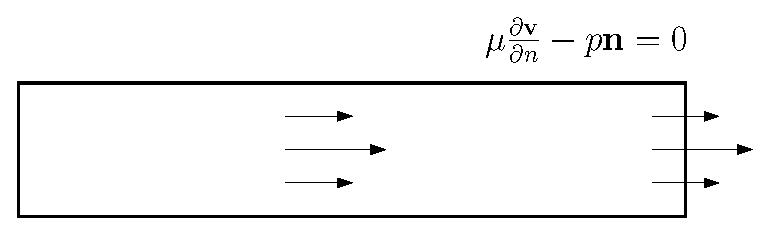
\includegraphics{figures/Pseudo_traction}
\caption{The pseudo traction boundary condition implies a continuation of the channel}
\label{fig:Pseudo_traction}
\end{figure}
\begin{figure}
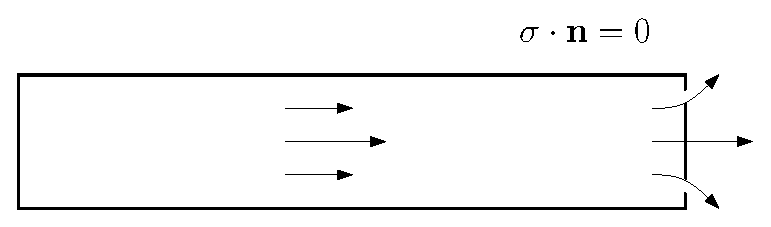
\includegraphics{figures/Boundary_force}
\caption{No external forces implies an open end of the channel, and fluid can escape in all directions}
\label{fig:Boundary_force}
\end{figure}
\end{center}
\clearpage
\section{Linear Elasticity}
The equations describing elasticity is derived by using Reynolds Transport theorem on a moving domain, $\Omega^t$, consisting of the same particles at all times. For conservation of momentum, the change in momentum must equal the applied forces to the system as well as body forces.  
\begin{align}
\mdi{}{t}\int_{\Omega^t} \rho \mathbf{v} \mathrm{d}V = \int_{\Omega^t} \rho \pdi{\mathbf{v}}{t} \mathrm{d}V + \int_{\partial \Omega^t} \rho \mathbf{v} \mathbf{v}\cdot \mathbf{n} \mathrm{d}S = \int_{\partial \Omega^t} \sigma_s \cdot \mathbf{n} \mathrm{d}S + \int_{\Omega^t}\mathbf{F}_v \mathrm{d}V
\end{align}
Where $\sigma_s$ is the stress tensor describing the elastic material. By applying Gauss' theorem again we end up with the general elasticity equation in a moving domain.
\begin{align}
\rho \pdi{\mathbf{v}}{t} + \rho( \mathbf{v} \cdot \nabla) \mathbf{v} = \nabla \cdot \sigma_s + \mathbf{F}_v \label{LE}
\end{align}
Linear elasticity is an approximation used for small deformations for elastic solids. As a rule of thumb the approximation of linear elasticity is usually valid for deformations up to 10\% relative to the solid. The stress tensor for a linear elastic medium is very similar to \eqref{Stress} describing an incompressible Newtonian fluid except there is no fluid pressure, and the stress is related to the total displacement $\mathbf{U}$ rather than the velocity $\mathbf{v}$. The stress tensor for such a material reads:
$\sigma_s = 2\mu\epsilon(\mathbf{U}) + \lambda \text{tr}(\epsilon(\mathbf{U}))$, where $\epsilon$ is defined exactly as the strain rate tensor for a Newtonian fluid. Usually, within the framework of linear elasticity, the convective term is also regarded as small and thus neglected. It is then common to write the equation only involving one unknown, $\mathbf{U}$.
\\
\\
We choose to keep the equation \eqref{LE} for simulations in this thesis. The reason for choosing the solid velocity $\mathbf{v}$ as the unknown will be discussed in chapter 5. Also, by using this form, the nonlinear term add no complexity to the coupled system we want to solve later, as the momentum equation in the fluid will have a similar term. Thus, our linear elasticity approximation lies in the inexact description of $\sigma_s$ which in general will consist of nonlinear terms depending on the elasticity model. \\ \\

\section{Linear Poroelasticity}
In this section, the equations describing fluid flowing trough an elastic, porous medium is presented. For a more detailed discussion, derivation and history within the field we refer to Wang \cite{Wang00} on Linear Poroelasticity. To keep the mathematics as similar to the fluid case as possible, we use $\mu$ and $\lambda$ instead of the possion ratio. The equations describing linear poroelasticity are often described as Biot's equations. 
\\
\\
\subsection{Fluid flow through a porous media}
A porous medium is a material with pores in which fluid can flow. The principles of modeling porous flow consist of macroscopic averaging over the pores. The material part is often known as the skeleton, matrix or frame and in general all the pores will have different size and shape. In this section the skeleton is assumed rigid. The nature of the material defines whether we will be able to fully solve the problem with no-slip conditions on all skeleton parts, or if some kind of volumetric averaging can be done. If the observer is interested in velocity variations on the scales of the pores, conventional fluid dynamics must be used. When there are many pores and channels, the complexity of the problem makes the full Navier-Stokes system difficult to solve. In these cases, macroscopic volume averaging is usually done, where the effects of the skeleton is modeled by introducing parameters constant over the material considered, such as permeability and conductivity. 
\\
These kinds of simplifications results in the famous Darcy's law (see e.g. Nield and Bejan \cite{Niel13}), here generalized in three dimensions
\begin{align}
\mathbf{q} = -\frac{1}{\mu} \mathbf{K} \cdot \nabla p \label{Darcy3}.
\end{align}
Here $\mathbf{K}$ is the \textit{permeability} tensor, and $\mu$ is the dynamic viscosity of the fluid. If the medium considered is isotropic, the permeability is a scalar value and equation \eqref{Darcy3} can be expressed as
\begin{align}
\mathbf{q} = -\frac{K}{\mu} \nabla p \label{Darcy}
\end{align}
Sometimes the permeability is given through the \textit{hydraulic conductivity}, $\kappa$, where $\kappa = \frac{K}{\mu_f}$ relates the two parameters for a fully saturated porous medium. It should be noted that the velocity $\mathbf{q}$ known as the Darcy velocity (or Darcy flux) represents the average flux over a representative elementary volume (r.e.v.), and thus the fluid velocity experienced by a particle in the pores will be $\mathbf{v}_p = \frac{\mathbf{q}}{\phi}$ where $\phi$ is the \textit{porosity} and describes the ratio of the pore volume versus the total volume. i.e. a high porosity indicates a large volume of pores compared to the skeleton and in general less obstruction of fluid.
\begin{center}
\begin{figure}[!ht]
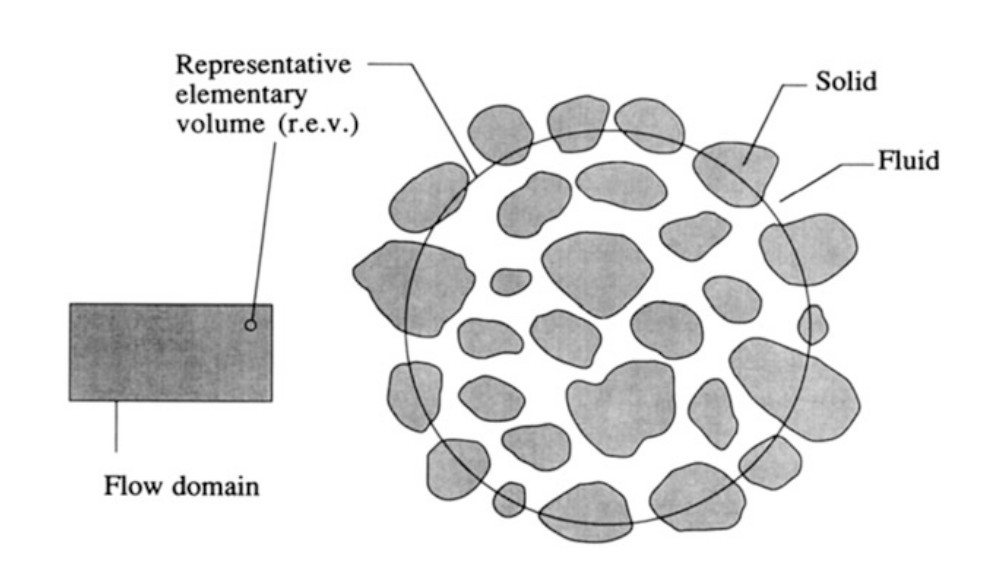
\includegraphics[scale=0.3]{figures/Porous_REV}
\caption{Representation of porous media where the averaging approach is used. From Nield and Bejan}
\end{figure}
\end{center}
\begin{center}
\begin{figure}[!ht]
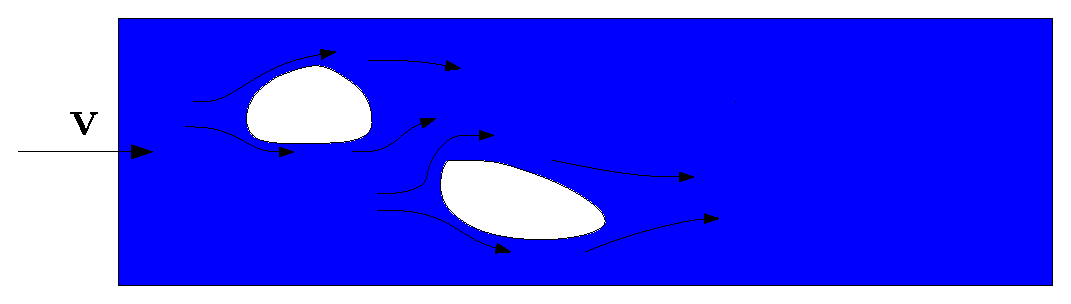
\includegraphics[width=0.9\linewidth]{figures/Porous_Islands}
\caption{River flow around two islands representing the pores. The full Navier-Stokes system should be solved for this problem}
\end{figure}
\end{center}
\subsection{Biot's equations} \label{sec:Biot}
As in the previous section, we let the domain consist of a skeleton with fluid filled pores. The extension for the Biot problem is that the skeleton is now free to move as an elastic material. Incompressibility for the fluid and solid is assumed. We define the filtration velocity $\mathbf{q} = \phi(\mathbf{v}_p - \mathbf{v}_s)$ where $\mathbf{v}_p$ is the fluid velocity in the pores and $\mathbf{v}_s$ is the structural velocity. $\mathbf{q}$ is thus regarded as the relative velocity of the fluid compared to the solid. The velocity of the skeleton $\mathbf{v}$, the filtration velocity $\mathbf{q}$, and the pore pressure $p$, can now be related by the following set of equations\cite{Biot41},\cite{Biot55},\cite{Biot72} 
\begin{alignat}
\rho \rho_p \mdi{\mathbf{v}_s}{t} + \rho_f \mdi{\mathbf{q}}{t} + \nabla p - \nabla \cdot \sigma_s(\mathbf{U}) \quad = \mathbf{f}_s \label{MomentumS}  \\
\rho_f \mdi{\mathbf{v}_s}{t} + \rho_f \mdi{\mathbf{q}}{t}\frac{1}{\phi} + K^{-1}\mathbf{q} + \nabla p \quad = \mathbf{f}_d \label{MomentumSF}\\
\nabla \cdot (\mathbf{v}_s + \mathbf{q}) \quad = 0 \label{ContinuityS}
\end{alignat}
These equations state conservation of momentum equation for the total force balance \eqref{MomentumS}, conservation of momentum for the fluid phase only, \eqref{MomentumSF} and the constraint of incompressibility \eqref{ContinuityS}. $\rho_f$ is the density of the fluid in the pores, and $\rho_p = \rho_s(1-\phi) + \rho_f \phi$ where $\rho_s$ is the density of the skeleton. 
\\
\\
In relation to Darcy's law without external forces, equation \eqref{MomentumSF} describes an extension both in terms of the material derivative of $\mathbf{q}$, as well as extension into the poroelastic regime. The former is an extension to Darcy's law as proposed by Nield and Bejan, where originally we have used $\frac{1}{\phi}$ as the acceleration coefficient tensor. Biot's equations have been much used in applied geoscience and hydrogeology, where the time derivative $\mdi{\mathbf{q}}{t}$ is small. This assumption is probably less valid for some applications within biomedical computing, however as the spinal cord has previously believed to be impermeable, and also according to previous results by Dr{\o}sdal \cite{Dros11}, we expect $\mathbf{q}$ to be small and that the material derivative can be dropped. The term $K^{-1}\mathbf{q}$ should be kept as $K$ is assumed to be comparable to $\mathbf{q}$ in orders of magnitude.


\section{Descriptions of Motion} \label{sec:DoM}
The conservation equations for Newtonian fluids were derived from Reynolds' transport theorem by using a control volume fixed in space, while for elastic materials a moving control volume was used. In addition, we saw for instance that the stress tensor for elastic solids were linked to the total displacement, or deviation from the stress-free configuration, in the material. The stresses and velocity in the material will depend on the current deformation of the material with respect to the stress-free configuration. 
\\To this end, it will be convenient to provide the reader with two classical descriptions of a continuum in motion. 
\subsection{Lagrangian and Eulerian descriptions of motion}
We consider a domain $\Omega_{\mathbf{X}} \in \mathbb{R}^3$ consisting of material particles $\mathbf{X}$. The domain can undergo deformations, and the deformed domain, $\Omega_{\textit{\textbf{x}}}$, is the current configuration at time $t$. 
\begin{center}
\begin{figure}[!ht]
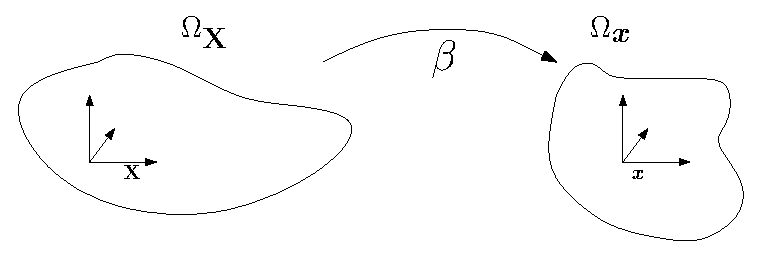
\includegraphics{figures/Lagrangian_domain} \label{Lagrangian}
\caption{Lagrangian description of motion. The mapping $\beta$ maps the reference coordinates to the spatial ones}
\end{figure}
\end{center}

We define the one-to-one mapping:
\begin{align}
\beta \,\, : \,\, \Omega_{\mathbf{X}} \times [0,T] \rightarrow  \Omega_{\mathbf{x}} \times [0,T] \\
(\mathbf{X},t) \rightarrow \beta(\mathbf{X},t) = (\mathbf{x},t)
\end{align}
Which takes any point $\mathbf{X}$ in the reference configuration to a new position $\mathbf{x} = \beta(\mathbf{X},t)$ at time $t$. As the mapping is one-to-one, it is also possible to keep track of the history of the motion by the inverse, $\beta^{-1}$. The time is measured with the same variable, $t$, in both domains. The gradient of $\beta$ with respect to $(\mathbf{X},t)$ can be written in matrix form as:
\begin{align}
\pdi{\beta}{(\mathbf{X},t)} = \begin{pmatrix} \pdi{\mathbf{x}}{\mathbf{X}} & \mathbf{v} \\
											0^T & 1
								\end{pmatrix} \label{betaGradient}
\end{align}
where the material velocity
\begin{align} \mathbf{v}(\mathbf{X},t) = \pdi{\mathbf{x}}{t}\Big{|}_{\mathbf{X}} \label{MatVel}
\end{align}
is the temporal change in the spatial variable $\mathbf{x}$ while holding \textbf{X} fixed. $0^T$ denotes a null vector. 
\\
The \textit{Lagrangian} description, where we follow a fixed set of material particles as suggested by the mapping $\beta$, is often used. In the Lagrangian description all quantities are expressed in terms of the reference configuration $\Omega_{\mathbf{X}}$ and time. In other words, even though the material is deformed, we can still compute displacements and particle velocities using the material coordinates $\mathbf{X}$. For instance, the displacement from the starting material configuration will be given as $\beta(\mathbf{X},t) - \mathbf{X}$ and the velocity as given in equation \eqref{MatVel}. \\ Because the grid coincides with the material coordinates, there are no convective terms in the Lagrangian description. In the context of Reynold's Transport theorem, the Lagrangian approach coincides with a moving control volume consisting of the same material points at all time. When a material undergoes large deformations or for instance vortices or turbulence occour, the material velocity from the Lagrangian point of view becomes difficult to handle. 
\\
\\
In fluid mechanics the \textit{Eulerian} description is the most used, which means that fluid flows through a fixed region in space and in each point we can measure various properties or quantities such as velocity, pressure and temperature. The conservation equations in the Eulerian description are expressed in terms of the spatial coordinates $\mathbf{x}$ and time, and are neither connected to a reference configuration nor the material coordinates. Compared to the Lagrangian approach, large material deformations is not a problem, as material can enter and leave the fixed domain. This movement of a material through a fixed region results in convective effects, and convection operators can often be problematic in computational fluid dynamics due to their non-symmetric nature. 
\\
\\
\subsection{The Arbitrary Eulerian Lagrangian description}
To be able to couple the Lagrangian approach for the solid with the Eulerian approach for the fluid, we need some referential system, not attached to the material points neither totally fixed in space. This type of description is common in FSI analysis and is known as the \textit{arbitrary Lagrangian-Eulerian} (ALE) description.
\\
\\The following derivation is inspired by the the works on Arbitrary Lagrangian-Eulerian methods by Donea et. al in \cite{Done04}. 
\\
\\
The need for an additional set of coordinates, an independent referential system with reference coordinates $\chi$ is introduced. This introduces two new mappings to relate all the different configurations as shown in fig. 
\begin{center}
\begin{figure}[!ht]
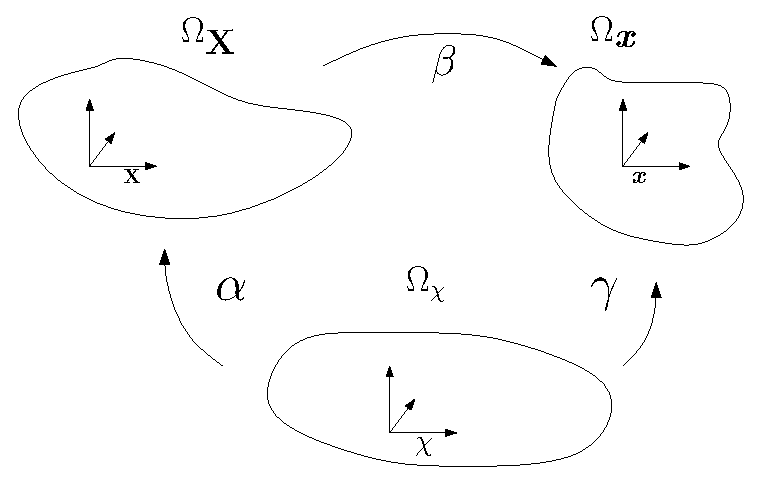
\includegraphics{figures/ALE_domain} \label{ALE_domain}
\caption{The three domains needed in the ALE formulation}
\end{figure}
\end{center}

The mappings are defined similarly to $\beta$ as
\begin{align}
\gamma \,\, : \,\, \Omega_{\chi} \times [0,T] \rightarrow  \Omega_{\mathbf{x}} \times [0,T] \\
(\chi,t) \rightarrow \gamma(\chi,t) = (\mathbf{x},t)
\end{align}
and the gradient of $\gamma$
\begin{align}
\pdi{\gamma}{(\chi,t)} = \begin{pmatrix} \pdi{\mathbf{x}}{\chi} & \mathbf{w} \\
											0^T & 1
								\end{pmatrix} \label{gammaGradient}
\end{align}
In addition, 
\begin{align} \mathbf{w}(\chi,t) = \pdi{\mathbf{X}}{t}\Big{|}_{\chi} \label{MeshVel}
\end{align}
denotes the mesh velocity. Both the mesh and the material can move independently of the laboratory. More precise, relative to some referential point in space, the fluid moves with veloctiy $\mathbf{v}$ and the domain moves with velocity $\mathbf{w}$. 
\\
\\
To complete the relation between the different velocities, we define the inverse of $\alpha$ directly: 
\begin{align}
\alpha^{-1} \,\, : \,\, \Omega_{\mathbf{X}} \times [0,T] \rightarrow  \Omega_{\chi} \times [0,T] \\
(\mathbf{X},t) \rightarrow \alpha^{-1}(\mathbf{X},t) = (\chi,t)
\end{align}
The gradient is given as
\begin{align}
\pdi{\alpha^{-1}}{(\mathbf{X},t)} = \begin{pmatrix} \pdi{\chi}{\mathbf{X}} & \mathbf{\hat{v}} \\
											0^T & 1
								\end{pmatrix} \label{alpha_Gradient}
\end{align}
Where the velocity 
\begin{align} \mathbf{\hat{v}}(\mathbf{X},t) = \pdi{\chi}{t}\Big{|}_{\mathbf{X}} \label{HatVel}
\end{align}
denotes the temporal change in the referential system while holding the material particle $\mathbf{X}$ fixed. Therefore the velocity $\mathbf{\hat{v}}$ can be interpereted as the particle velocity in the referential domain. \\
\\
We use that $\beta = \gamma \, \circ \, \alpha^{-1} = \gamma(\alpha^{-1}(\mathbf{X},t))$ and obtain a relation between the different velocities by differentiating $\beta$. 
\begin{align}
\pdi{\beta}{(X,t)}(\mathbf{X},t) & = \pdi{\gamma}{(\chi,t)}(\alpha^{-1}(\mathbf{X,t}))\, \pdi{\alpha^{-1}}{(\mathbf{X},t)}(\mathbf{X},t) \\
& = \pdi{\gamma}{(\chi,t)}(\chi,t)\, \pdi{\alpha^{-1}}{(\mathbf{X},t)}(\mathbf{X},t)
\end{align}
In matrix form this equation is written:
\begin{align}
	\begin{pmatrix} \pdi{\mathbf{x}}{\mathbf{X}} & \mathbf{v} \\
											0^T & 1
	\end{pmatrix} 
	= 
	\begin{pmatrix} \pdi{\mathbf{x}}{\chi} & \mathbf{w} \\
											0^T & 1
	\end{pmatrix}
	\begin{pmatrix} \pdi{\chi}{\mathbf{X}} & \mathbf{\hat{v}} \\
											0^T & 1
	\end{pmatrix}
\end{align}
After block-multiplication of the right hand side we end up with an equation relating all the different velocities:
\begin{align}
\mathbf{v} = \pdi{\mathbf{x}}{\chi}\cdot \mathbf{\hat{v}} + \mathbf{w}
\end{align}
To this end, it is convenient to define the convective velocity
\begin{align}
\mathbf{c}:= \mathbf{v}-\mathbf{w} = \pdi{\mathbf{x}}{\chi}\cdot \mathbf{\hat{v}}
\end{align}
which is the relative velocity between the material and the mesh. 
\\
\\
To obtain relation between quantities to formulate the balance equations, we let a scalar quantity, $Q$ be defined as $Q(\mathbf{x},t), Q^*(\chi,t)$ and $Q^{**}(\mathbf{X},t)$ in the spatial, referential and material domains respectively. \\
\\
To obtain a relation between the spatial description, $Q$, and material description $Q^{**}$ we can utilize the previously described mapping $\beta$:

\begin{align}
Q^{**}(\mathbf{X},t) = Q(\beta(\mathbf{X},t),t) = Q \, \circ \, \beta
\end{align}

The gradient of $Q^{**}$ can then be computed as
\begin{align}
\pdi{Q^{**}}{(\mathbf{X},t)}(\mathbf{X},t) = \pdi{Q}{(\mathbf{x},t)}(\mathbf{x},t) \, \pdi{\beta}{(\mathbf{X},t)}(\mathbf{X},t)  \label{Grad_Q}
\end{align}

\begin{align}
	\begin{pmatrix} \pdi{Q^{**}}{\mathbf{X}} & \pdi{Q^{**}}{t}
	\end{pmatrix}
	= 
	\begin{pmatrix} \pdi{Q}{\mathbf{x}} & \pdi{Q}{t}
	\end{pmatrix}
	\begin{pmatrix} \pdi{\mathbf{x}}{\mathbf{X}} & \mathbf{v} \\
											0^T & 1
	\end{pmatrix} \label{Matrix_Q}
\end{align}
After multiplication one can obtain the well known equation between material and spatial time derivaties:
\begin{align}
\pdi{Q^{**}}{t} = \pdi{Q}{t} + \pdi{Q}{\mathbf{x}} \cdot \mathbf{v} \label{Mat_Spa}
\end{align}
To ease notation we now recognize the material and spatial time derivatives $\pdi{Q^{**}}{t} = \pdi{Q}{t}\Big{|}_{\mathbf{X}}$, $\pdi{Q}{t} = \pdi{Q}{t}\Big{|}_{\mathbf{x}}$, and define the material and spatial derivatives the following way
\begin{align}
\frac{\mathrm{d}}{\mathrm{dt}} := \pdi{}{t}\Big{|}_{\mathbf{X}} \hspace{3cm} \pdi{}{t} := \pdi{}{t}\Big{|}_{\mathbf{x}}
\end{align}
The relation \eqref{Mat_Spa} can now be written in a form probably already known to the reader
\begin{align}
\frac{\mathrm{d}Q}{\mathrm{dt}} = \pdi{Q}{t} + (\mathbf{v} \cdot \nabla) Q \label{Material_derivative}
\end{align}
The next step is to relate the material and the referential description of the quantity, $Q^{**}$ and $Q^*$ respectively, by the mapping $\alpha$. This relation is written as 
\begin{align}
Q^{**} = Q^* \, \circ \, \alpha^{-1}
\end{align}
By proceeding the exact same way as way as in \eqref{Grad_Q} and \eqref{Matrix_Q} the relation between material and referential time derivatives is written
\begin{align}
\pdi{Q^{**}}{t} = \pdi{Q^*}{t} + \pdi{Q^*}{\chi}\cdot \mathbf{\hat{v}}
\end{align}
If we rather want to express the spatial derivative of $Q^*$ in the spatial domain, we can use the definition of $\mathbf{\hat{v}}$ from equation \eqref{HatVel} to end up with
\begin{align}
\pdi{Q^{**}}{t} = \pdi{Q^*}{t} + \pdi{Q}{\mathbf{x}} \cdot \mathbf{c}
\end{align}
This equation can be written in more common notation, and the following is known as \textit{The fundamental ALE equation}
\begin{align}
\frac{\mathrm{d}Q}{\mathrm{dt}} = \pdi{Q}{t}\Big{|}_{\chi} + (\mathbf{c} \cdot \nabla) Q \label{Fundamental_ALE}
\end{align}
and states that the time derivative in the material configuration equals its local (referential) derivative plus a convective term taking into account the relative difference in velocity between the two systems. It should be noted that the relations presented also holds for vector quantities. 
\\
\\
Also, by combining equations \eqref{Material_derivative} and \eqref{Fundamental_ALE}, we can relate the spatial time derivative with the referential time derivative as
\begin{align}
\pdi{Q}{t} = \pdi{Q}{t}\Big{|}_{\chi} - (\mathbf{w} \cdot \nabla) Q \label{Spatial_referential}
\end{align}



\section{Balance equations in the ALE framework}
To obtian appropriate balance equations in the ALE framework we start by noting that the balance equations can be written in terms of the material derivates as
\begin{align}
\frac{\mathrm{d}\rho}{\mathrm{dt}} = \pdi{\rho}{t} + \mathbf{v} \cdot \nabla \rho= -  \rho \cdot \nabla \mathbf{v}
\end{align}
\begin{align}
\rho \frac{\mathrm{d}\mathbf{v}}{\mathrm{dt}} = \rho \Big{(} \pdi{\mathbf{v}}{t} + (\mathbf{v} \cdot \nabla ) \mathbf{v} \Big{)} = \nabla \cdot \sigma
\end{align}
By using equation \eqref{Spatial_referential}, the spatial time derivatives can be replaced to obtain equations for the ALE framework. The following equations should hold in \textit{any} time-dependent domain which does not neccessarily need to coincide with the movement of material particles. 
\begin{align}
\pdi{\rho}{t}\Big{|}_\chi + \mathbf{c} \cdot \nabla \rho= -  \rho \nabla \cdot \mathbf{v} \quad \text{ in } \Omega^t \\
\rho \Big{(} \pdi{\mathbf{v}}{t}\Big{|}_\chi + (\mathbf{c} \cdot \nabla ) \mathbf{v} \Big{)} = \nabla \cdot \sigma \quad \text{ in } \Omega^t
\end{align}
Which shows that all one have to do in order to transform the Eulerian form of the balance equations into the ALE formulation is to replace the convective velocity with the relative velocity between the material and the mesh. 
\subsection{Mesh updating}
The velocity $\mathbf{w}$ can be seen as the mesh velocity when a computational mesh is used. In FSI, the ALE framework provides flexibility to combine the Lagrangian and Eulerian descriptions of motion. On the structural part, as well as on the fluid-structure interface, the domain $\Omega_s$ consists of the same material particles at all times and moves exactly with the material points within the structure. That is, $\mathbf{v}_s = \mathbf{w}_s$. The fluid domain has to follow the changes on the fluid-structure interface. Other than that the mesh velocity in the fluid domain is arbitrary in principle, but the choice of mesh velocity in the fluid domain is important for the accuracy of the solver. In general, important aspects to consider is disortion and squeeze of each element in the fluid domain. \\
\\
A Laplacian smoothing algorithm is used to update the mesh, consisting of solving a Laplace (or Poisson) equation for the mesh displacement in the fluid. The method is a mesh regularization method where the lines in the mesh have equal potential. This method was first introduced by Winslow in 1963 \cite{Wins63}.
\section{Fluid Structure Interaction}
By establishing the flexibility of the ALE formulation together with an equation for a moving domain we can now state the governing equations for the Fluid-Structure interaction problem. In the case of an Newtonian incompressible fluid together with a linear elastic material in the abscence of body forces, the mathematical problem consists of solving
\begin{alignat}{3}
\rho_f \Big{(} \pdi{\mathbf{v}}{t} + ((\mathbf{v}-\mathbf{w})  \cdot \nabla )  \mathbf{v} \Big{)} - \nabla \cdot \sigma_f(\mathbf{v},p)& = 0 \quad && \text{ in } \Omega_f^t \\
\nabla \cdot \mathbf{v} & = 0 && \text{ in } \Omega_f^t\\
\nabla ^2 \mathbf{U} & = 0 && \text{ in } \Omega_f^t
\\
\\
\rho_s \pdi{\mathbf{v}}{t} + \rho_s(\mathbf{v}\cdot\nabla)\mathbf{v} -\nabla \cdot \sigma_s(\mathbf{U}) & = 0  &&\text{ in } \Omega_s^t \\
\mathbf{w} & =  \mathbf{v} && \text{ in } \Omega_s^t
\end{alignat}
In the case of fluid interacting with a solid structure, no material can cross the moving boundary $\Gamma^t$, and thus the fluid and solid velocity must be equal on the interface between the fluid and the solid. In general, one have to ensure mass conservation on the boundary. In addition the forces acting on the surface must be equal. A difference in forces from each material on the interface would result in infinite acceleration on the infinitely thin surface. Mathematicly, these two conditions can be stated as
\begin{align}
\begin{rcases}
\sigma_f \cdot \mathbf{n} & =  \sigma_s \cdot \mathbf{n} \\
\mathbf{v}_f & = \mathbf{v}_s
\end{rcases}
\text{ on } \Gamma^t
\end{align}
And will be used at all interfaces in FSI simulations. Kinematic or dynamic boundary conditions will be needed on the other boundaries as well, but will differ depending on the problem considered. 
\\

\section{Coupling Fluid Flow with Poroelasticity}
In a similar fashion to the Fluid-Structure interaction problem, and with the simplifications assuming the filtration velocity is small, the Biot problem together with Navier-Stokes equations consists of solving
\begin{alignat}{3}
\rho_f \Big{(} \pdi{\mathbf{v}_f}{t} + ((\mathbf{v}_f-\mathbf{w})  \cdot \nabla )  \mathbf{v}_f \Big{)} - \nabla \cdot \sigma_f(\mathbf{v}_f,p_f)& =  0 \quad  && \text{ in } \Omega_f^t \\
\nabla \cdot \mathbf{v}_f & = 0 && \text{ in } \Omega_f^t\\
\nabla ^2 \mathbf{U} & = 0 && \text{ in } \Omega_f^t
\\
\\
\rho_p \pdi{\mathbf{v}_s}{t} + \rho_p(\mathbf{v}_s\cdot\nabla)\mathbf{v}_s - \nabla \cdot \sigma_s(\mathbf{U}) + \nabla p_s & =  0 && \text{ in } \Omega_s^t \\
\rho_p \pdi{\mathbf{v}_s}{t} + \rho_p(\mathbf{v}_s\cdot\nabla)\mathbf{v}_s + K^{-1}\mathbf{q} + \nabla p_s & =  0 && \text{ in } \Omega_s^t \\
\nabla \cdot (\mathbf{v}_s + \mathbf{q}) & = 0 && \text{ in } \Omega_s^t \\
\end{alignat}

Boundary conditions at the interface for the given problem have been discussed over the years, and in 1967 Beavers and Joseph \cite{Beav67} published a paper describing experiments investigating the slip rate at a horizontal permeable wall located at y=0 with fluid flow above the porous medium. The boundary condition at the wall y=0 should be
\begin{align}
\pdi{v_f}{y} = \frac{\alpha_{\text{BJ}}}{K^{1/2}}(v_f-q), \label{BJ}
\end{align}
where $v_f$ is the fluid velocity tangential to the plane, $q$ is the seepage or filtration velocity in the porous medium, K is the permeability and $\alpha_{\text{BJ}}$ is a constant depending on the material parameters of the porous medium close to the boundary. The derivative on the left hand side of equation \eqref{BJ} should be evaluated just above the plane and $q$ should be evaluated just below the plane. 
In 1971 Saffmann \cite{Saff71} generalized the problem to other geometries as well as showing that the filtration velocity $q$ could be left out of the equation only adding errors of order $O(K)$. Jones, (1973) \cite{Jone73} assumed shortly afterwards that the velocity jump was proportional to the shear stress rather than velocity shear. These additions to the original boundary condition proposed by Beavers and Joseph (known as the Beavers-Joseph-Saffmann (BSJ) condition) was used in spinal canal models by Dr{\o}sdal:
\begin{align}
2\mathbf{n} \cdot \epsilon(\mathbf{v}_f) \cdot \tau = \alpha_{\text{BJ}}K^{-1/2}\mathbf{v}_f\cdot \tau \label{BJS}
\end{align}
and showed to have minimal effect on key value measurements such as filtration velocity in the cord as well as fluid veloctiy in both the SAS and inside the syrinx. (Values changed by $10^{-4} \%$ for $\alpha_{\text{BJ}}$ ranging from 0 to 1). This condition is therefore omitted in this thesis. 
\\
\\
As in the FSI case, we assume conservation of mass and continuity of stresses at the interface. The boundary condition is related through the velocities and the Darcy flux at the boundary. 
\begin{align}
\begin{rcases}
\mathbf{v}_f & = \mathbf{v}_s + \mathbf{q} \\
\sigma_f \cdot \mathbf{n} & =  \sigma_s \cdot \mathbf{n} - p_p\mathbf{n}
\end{rcases} 
\text{ on } \Gamma^t \label{Biotbnd}
\end{align}
Strictly speaking, mass conservation does not neccessarily imply the tangential velocitites to be continuous at the interface, and the transition in tangential velocity is what the BJS-condition tries to capture. However, as we shall see later, with the limitiations by using continous functions in the computational modeling the tangential velocities will also have to be continuous. This limitation is also the case for the pressure, and as pointed out by Nield and Bejan (2013) \cite{Niel13} these assumptions together with the BJS-condition results in an overdetermined system. The pressure will be continuous on the microscopic scale, but only approximately continuous on the macroscopic (averaging) scale. Despite these limitations, we stick with the boundary conditions \eqref{Biotbnd} assuming, as showed on porous flow, the BJS-condition barely alters the solution. 
